In questa sezione vengono presentati i casi d\textquoteright{}uso al fine di riassumere in un linguaggio intuitivo e di facile comprensione (UML2.0) ci\`{o} che il capitolato richiede. Questa non \`{e} da ritenersi un\textquoteright{}analisi completa, in quanto il prodotto se verr\`{a} sviluppato risponder\`{a} ad un numero maggiore di funzionalit\`{a} rispetto a quelle qui presentate e di questo la pianificazione ne terr\`{a} conto, in particolare dal punto di vista di costi e scadenze di consegna.

\subsection{Casi d'uso}

\subsubsection[UC0: Scenario principale]{UC0: Scenario principale}
\begin{figure}[H]
  \begin{center}
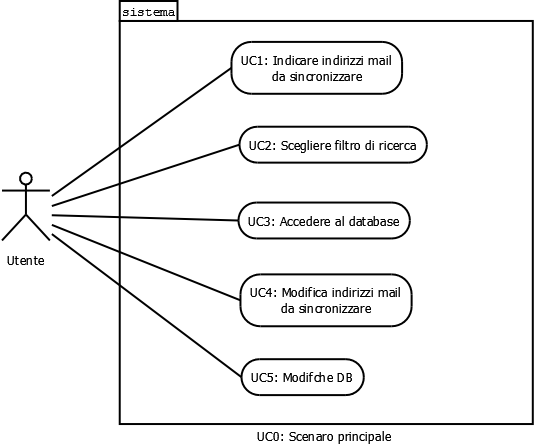
\includegraphics[width=0.60\textwidth]{img/UC0_ScenarioPrincipale.png}
\caption{UC0: Scenario principale}
\label{fig:UC0}
\end{center}
\end{figure}

\begin{description}
\item[Attori:]{utente.}
\item[Precondizione:]{il sistema visualizza la schermata iniziale dell\textquoteright{}applicativo e le infrastrutture di rete sono funzionanti.}
\item[Scenario principale:]{l\textquoteright{}utente accedendo all\textquoteright{}applicazione pu\`{o} eseguire le seguenti operazioni:
	\begin{itemize}
	\item \textbf{Indicare gli indirizzi mail da sincronizzare}: l\textquoteright{}utente pu\`{o} scegliere per quali indirizzi mail \`{e} interessato memorizzare le newsletter (UC0.1);
	\item \textbf{Scegliere filtro di ricerca}: l\textquoteright{}utente pu\`{o} scegliere dei criteri di ricerca per visualizzare i dati sul database: esso pu\`{o} visualizzare per esempio newsletter inviate presso un certo indirizzo mail, piuttosto che per data o per fornitore (UC0.2);
	\item \textbf{Accedere al database}: l\textquoteright{}utente potr\`{a} confermare il criterio di ricerca scelto e visualizzare cos\`{i} le informazioni memorizzate nel database che soddisfano la query di ricerca e quindi il sistema provveder\`{a} a visualizzare quanto chiesto dall\textquoteright{}utente (UC0.3);
	\item \textbf{Modifica indirizzi mail da sincronizzare}: l\textquoteright{}utente pu\`{o} scegliere di modificare gli indirizzi mail configurati nella sincronizzazione (UC0.4);
	\item \textbf{Modifiche DB}: l\textquoteright{}utente pu\`{o} scegliere di effettuare operazioni di modifica a parte delle informazioni memorizzate nel database(UC0.5);	
	\end{itemize}}
\item[Postcondizione per successo:]{il sistema \`{e} in attesa di una scelta da parte dell\textquoteright{}utente.}
\end{description}

\subsubsection[UC4: Modifica indirizzi mail da sincronizzare]{UC4: Modifica indirizzi mail da sincronizzare}
\begin{figure}[H]
  \begin{center}
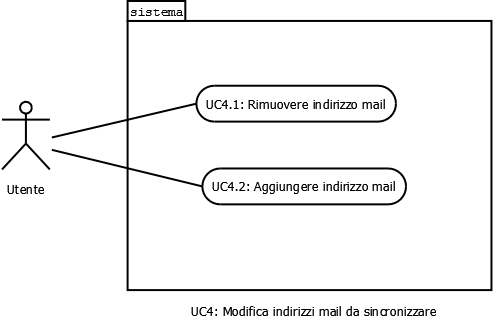
\includegraphics[width=0.60\textwidth]{img/UC4_ModificaIndirizziMailDaSincronizzare.png}
\caption{UC4: Modifica indirizzi mail da sincronizzare}
\label{fig:UC4}
\end{center}
\end{figure}

\begin{description}
\item[Attori:]{utente.}
\item[Precondizione:]{il sistema ha caricato gli indirizzi mail scelti per la configurazione e li visualizza, le infrastrutture di rete sono funzionanti.}
\item[Scenario principale:]{l\textquoteright{}utente pu\`{o} eseguire le seguenti operazioni:
	\begin{itemize}
	\item \textbf{Rimuovere indirizzi mail}: l\textquoteright{}utente pu\`{o} scegliere quali indirizzi mail rimuovere dalla sincronizzazione e quindi il sistema provveder\`{a} alla rimozione delle newsletter inviate presso quello specifico indirizzo mail (UC4.1);
	\item \textbf{Aggiungere indirizzi mail}: l\textquoteright{}utente pu\`{o} scegliere quali indirizzi mail aggiungere alla sincronizzazione (UC4.2);
	\end{itemize}}
\item[Postcondizione per successo:]{il sistema ha aggiornato gli indirizzi mail da sincronizzare.}
\end{description}

\subsubsection[UC5: Modifiche DB]{UC5: Modifiche DB}
\begin{figure}[H]
  \begin{center}
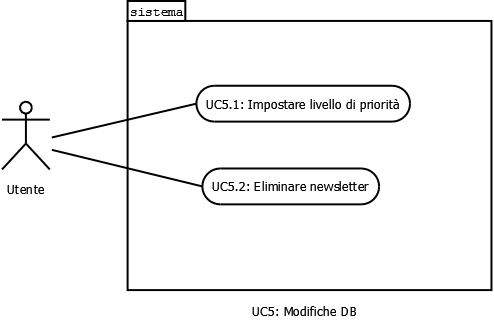
\includegraphics[width=0.60\textwidth]{img/UC5_ModificheDB.png}
\caption{UC5: Modifiche DB}
\label{fig:UC5}
\end{center}
\end{figure}

\begin{description}
\item[Attori:]{utente.}
\item[Precondizione:]{il sistema ha caricato le newsletter risultato dei filtri di ricerca scelti dall\textquoteright{}utente.}
\item[Scenario principale:]{l\textquoteright{}utente pu\`{o} eseguire le seguenti operazioni:
	\begin{itemize}
	\item \textbf{Impostare un livello di priorit\`{a}}: l\textquoteright{}utente pu\`{o} scegliere di attribuire un livello di priorit\`{a} ad una certa newsletter (UC5.1);
	\item \textbf{Rimuovere newsletter}: l\textquoteright{}utente pu\`{o} scegliere quali newsletter rimuovere (UC5.2);
	\end{itemize}}
\item[Postcondizione per successo:]{il sistema ha aggiornato le modifiche alle newsletter effettuate dall\textquoteright{}utente.}
\end{description}

\subsection{Requisiti funzionali}

\subsubsection{Obbligatori}

\begin{description}
\item[RF.ob.1:] Il software deve permettere all\textquoteright{}utente di indicare gli indirizzi mail da sincronizzare.
\item[RF.ob.2:] Il software deve permettere all\textquoteright{}utente di modificare gli indirizzi mail che ha deciso di sincronizzare.
\begin{description}
\item[RF.ob.2.1:] Il software deve permettere all\textquoteright{}utente di aggiungere un indirizzo mail per la sincronizzazione.
\item[RF.ob.2.2:] Il software deve permettere all\textquoteright{}utente di rimuovere un indirizzo mail dalla sincronizzazione.
\begin{description}
\item[RF.ob.2.2.1:] Il software deve rimuovere le newsletter ricevute all\textquoteright{}indirizzo mail eliminato dalla sincronizzazione.
\end{description}
\end{description}
\item[RF.ob.3:] Il software deve permettere all\textquoteright{}utente di selezionare la mail o le mail per le quali visualizzare le newsletter ricevute.
\begin{description}
\item[RF.ob.3.1:] Il software deve permettere all\textquoteright{}utente di visualizzare la data in cui \`{e} stata ricevuta la newsletter.
\item[RF.ob.3.2:] Il software deve permettere all\textquoteright{}utente di visualizzare il titolo delle newsletter.
\item[RF.ob.3.3:] Il software deve permettere all\textquoteright{}utente di visualizzare il contenuto delle newsletter.
\item[RF.ob.3.4:] Il software deve permettere all\textquoteright{}utente di visualizzare il fornitore del prodotto promosso nella newsletter.
\item[RF.ob.3.5:] Il software deve permettere all\textquoteright{}utente di visualizzare il contenuto del prodotto promosso nella newsletter.
\item[RF.ob.3.5:] Il software deve permettere all\textquoteright{}utente di visualizzare la fonte del prodotto promosso nella newsletter.
\item[RF.ob.3.6:] Il software deve permettere all\textquoteright{}utente di visualizzare l\textquoteright{}immagine del prodotto promosso nella newsletter.
\item[RF.ob.3.7:] Il software deve permettere all\textquoteright{}utente di modificare il database.
\begin{description}
\item[RF.ob.3.7.1:] Il software deve permettere all\textquoteright{}utente di eliminare dal database una newsletter.
\end{description}
\end{description}
\end{description}

\subsubsection{Desiderabili}

\begin{description}
\item[RF.de.1:] Il software deve permettere all\textquoteright{}utente di assegnare una priorit\`{a} alle newsletter.
\begin{description}
\item[RF.de.1.1:] Il software deve permettere all\textquoteright{}utente di assegnare dei valori di priorit\`{a} da 1 a 5.
\begin{description}
\item[RF.de.1.1.1:] Un valore di priorit\`{a} pari a 1 dovr\`{a} indicare un valore di scarsissima priorit\`{a}.
\item[RF.de.1.1.2:] Un valore di priorit\`{a} pari a 2 dovr\`{a} indicare un valore di bassa priorit\`{a}.
\item[RF.de.1.1.3:] Un valore di priorit\`{a} pari a 3 dovr\`{a} indicare un valore di normale priorit\`{a}.
\item[RF.de.1.1.4:] Un valore di priorit\`{a} pari a 4 dovr\`{a} indicare un valore di media priorit\`{a}.
\item[RF.de.1.1.5:] Un valore di priorit\`{a} pari a 5 dovr\`{a} indicare un valore di alta priorit\`{a}.
\end{description}
\end{description}
\item[RF.de.2:] Il software deve permettere di effettuare delle visualizzazioni di newsletter filtrando in base a criteri di ricerca scelti dall\textquoteright{}utente.
\begin{description}
\item[RF.de.2.1:] Il software deve permettere di filtrare le newsletter per indirizzi mail.
\item[RF.de.2.2:] Il software deve permettere di filtrare le newsletter per data.
\item[RF.de.2.3:] Il software deve permettere di filtrare le newsletter per priorit\`{a}.
\item[RF.de.2.4:] Il software deve permettere di filtrare le newsletter per fonte.
\item[RF.de.2.5:] Il software deve permettere di filtrare le newsletter per fornitore.
\end{description}
\end{description}
 
